\begin{frame}
    \frametitle{Traditional grids}
    \begin{columns}
    \begin{column}{0.6\linewidth}
    \centering

    \vspace{10mm}

    \begin{itemize}
        \item Spherical grids
        \item Good accuracy with \textbf{few} grid points
        \item Based on atomic symmetry
        \item Fitted to important properties like total energy and geometry
        \item Possibly less accurate for higher order properties
        \item Decomposed into atomic contributions
    \end{itemize}

    \vspace{2mm}

    \begin{equation}
        \nonumber
        \int F(r) dr \approx \sum_K^{atoms} \sum_i^{grid} \omega_K(r_i) F(r_i)
    \end{equation}

    \vspace{15mm}

    \scriptsize
    A. D. Becke, 
    {\it JCP}, \textbf{88} (4), 1988\\
    O. Treutler, R. Ahlrichs,
    {\it JCP}, \textbf{102} (1), 1995\\
    R. E. Stratman {\it et. al.}
    {\it Chem. Phys. Lett.}, \textbf{257}, 1996
    
    \end{column}

    \begin{column}{0.4\linewidth}
    \centering
    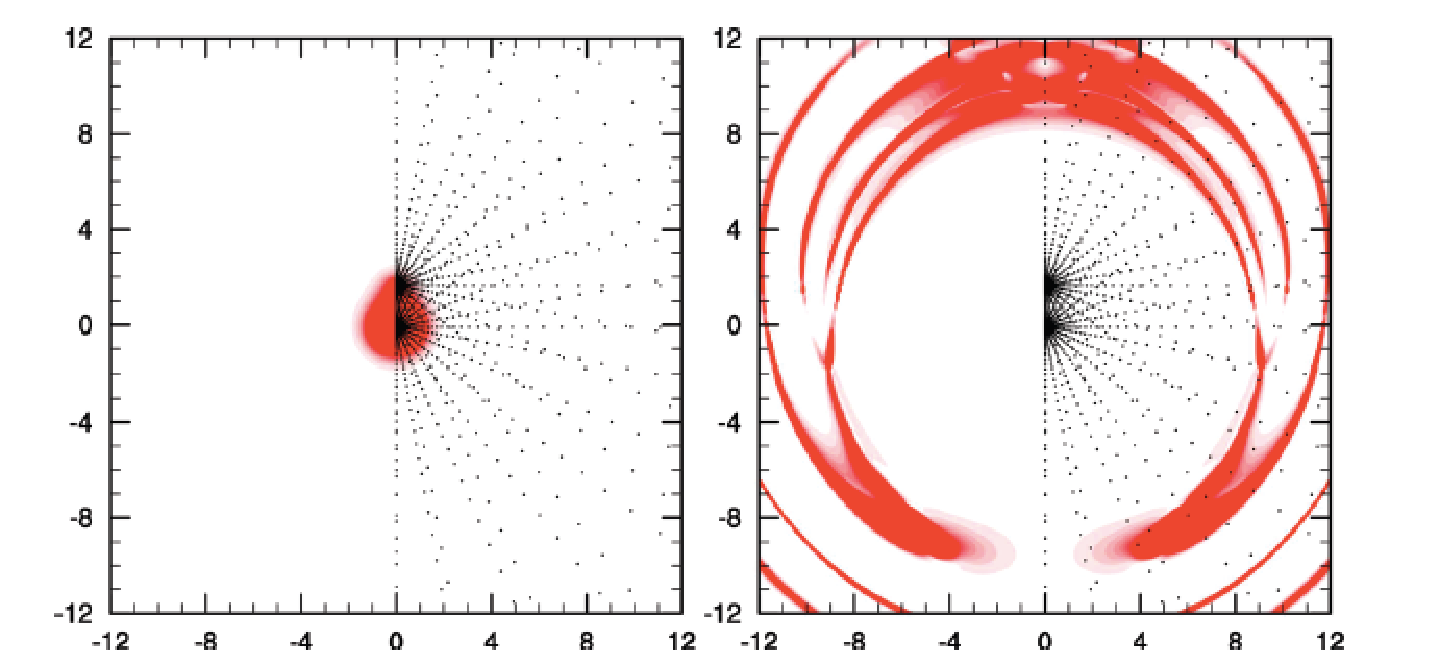
\includegraphics[clip, viewport = 0 0 650 350, angle=-90, scale=0.3]{figures/radialgrid.pdf}

    \vspace {2mm}

    \scriptsize
    U. Ekstr\"{o}m, {\it et. al.}
    {\it JCTC}, \textbf{6} (7), 2010
    \end{column}
    \end{columns}
\end{frame}

\begin{frame}
    \frametitle{MultiResolution Grids}
    \begin{columns}
    \begin{column}{0.5\linewidth}
    \begin{itemize}
        \item Cartesian grids
        \item Not constructed for specific properties
        \item Guaranteed accuracy with \textbf{many} grid points
        \item Can be individually fitted to each function
        \item Decomposed into cubic cells
    \end{itemize}

    \vspace{5mm}

    \begin{equation}
        \nonumber
        \int F(r) dr \approx \sum_K^{cells} \sum_i^{grid} \omega_K(r_i) F(r_i)
    \end{equation}
    \end{column}

    \begin{column}{0.5\linewidth}
    \centering
    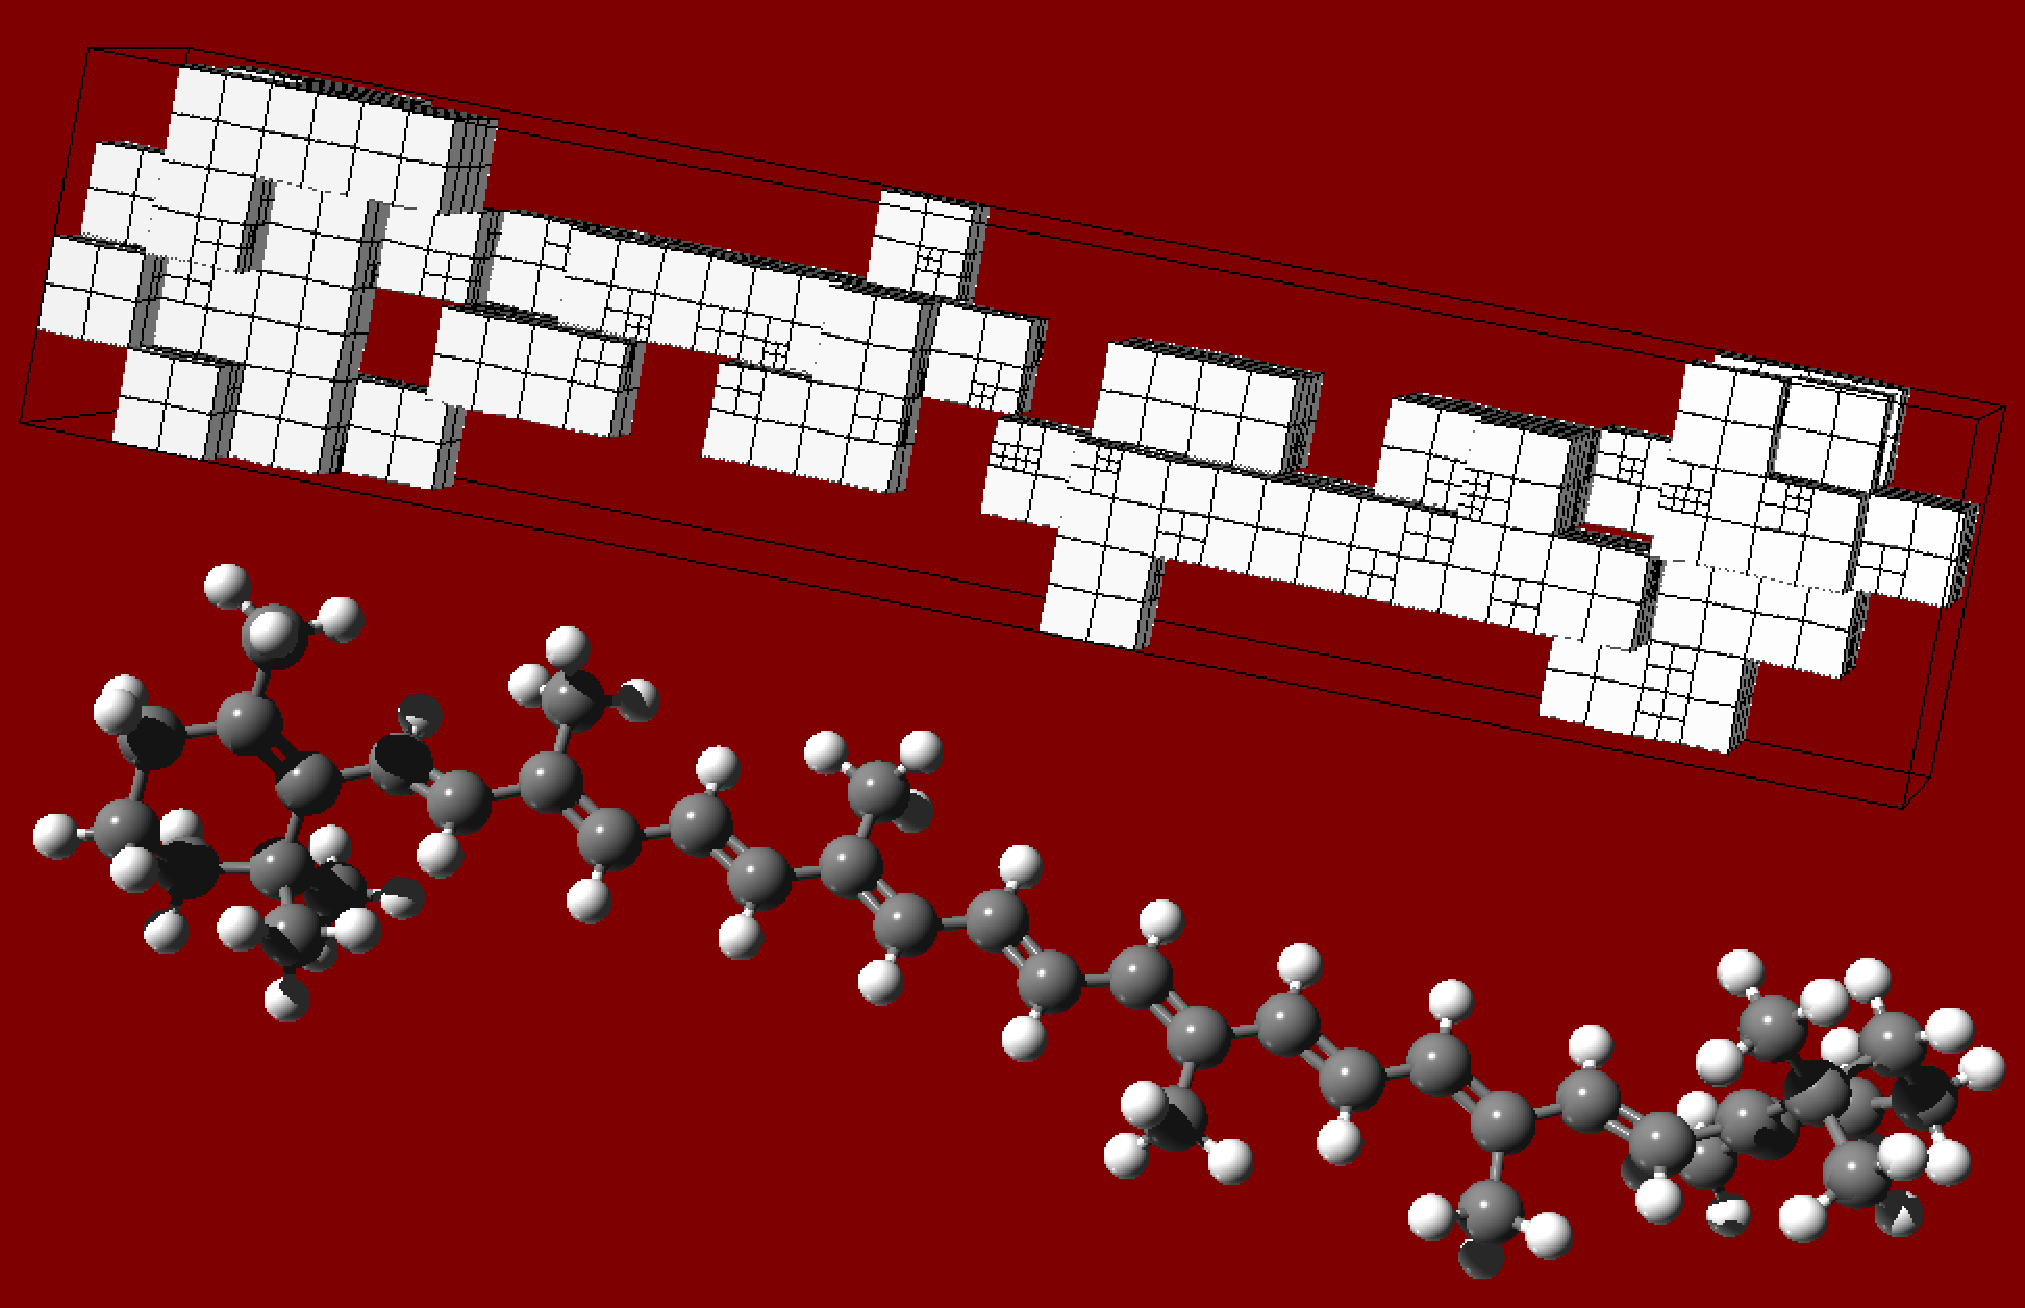
\includegraphics[angle=-90, scale=0.2]{figures/caroteneGrid.pdf}
    \end{column}
    \end{columns}
\end{frame}

